\subsection{Item Scanner Application}
The next two application were built on top of the deployed infrastructure from the energy audit.
The item scanner application shows a power trace of an item.  If the item is a space, it shows
the aggregate consumption of the space over a 24-hour period.  Figure~\ref{fig:itemscanscreen}
shows a screenshot of a trace for a room in on of the spaces we monitored.

%FILL IN WITH REAL GRAPH
\begin{figure}[htb!]
\begin{center}
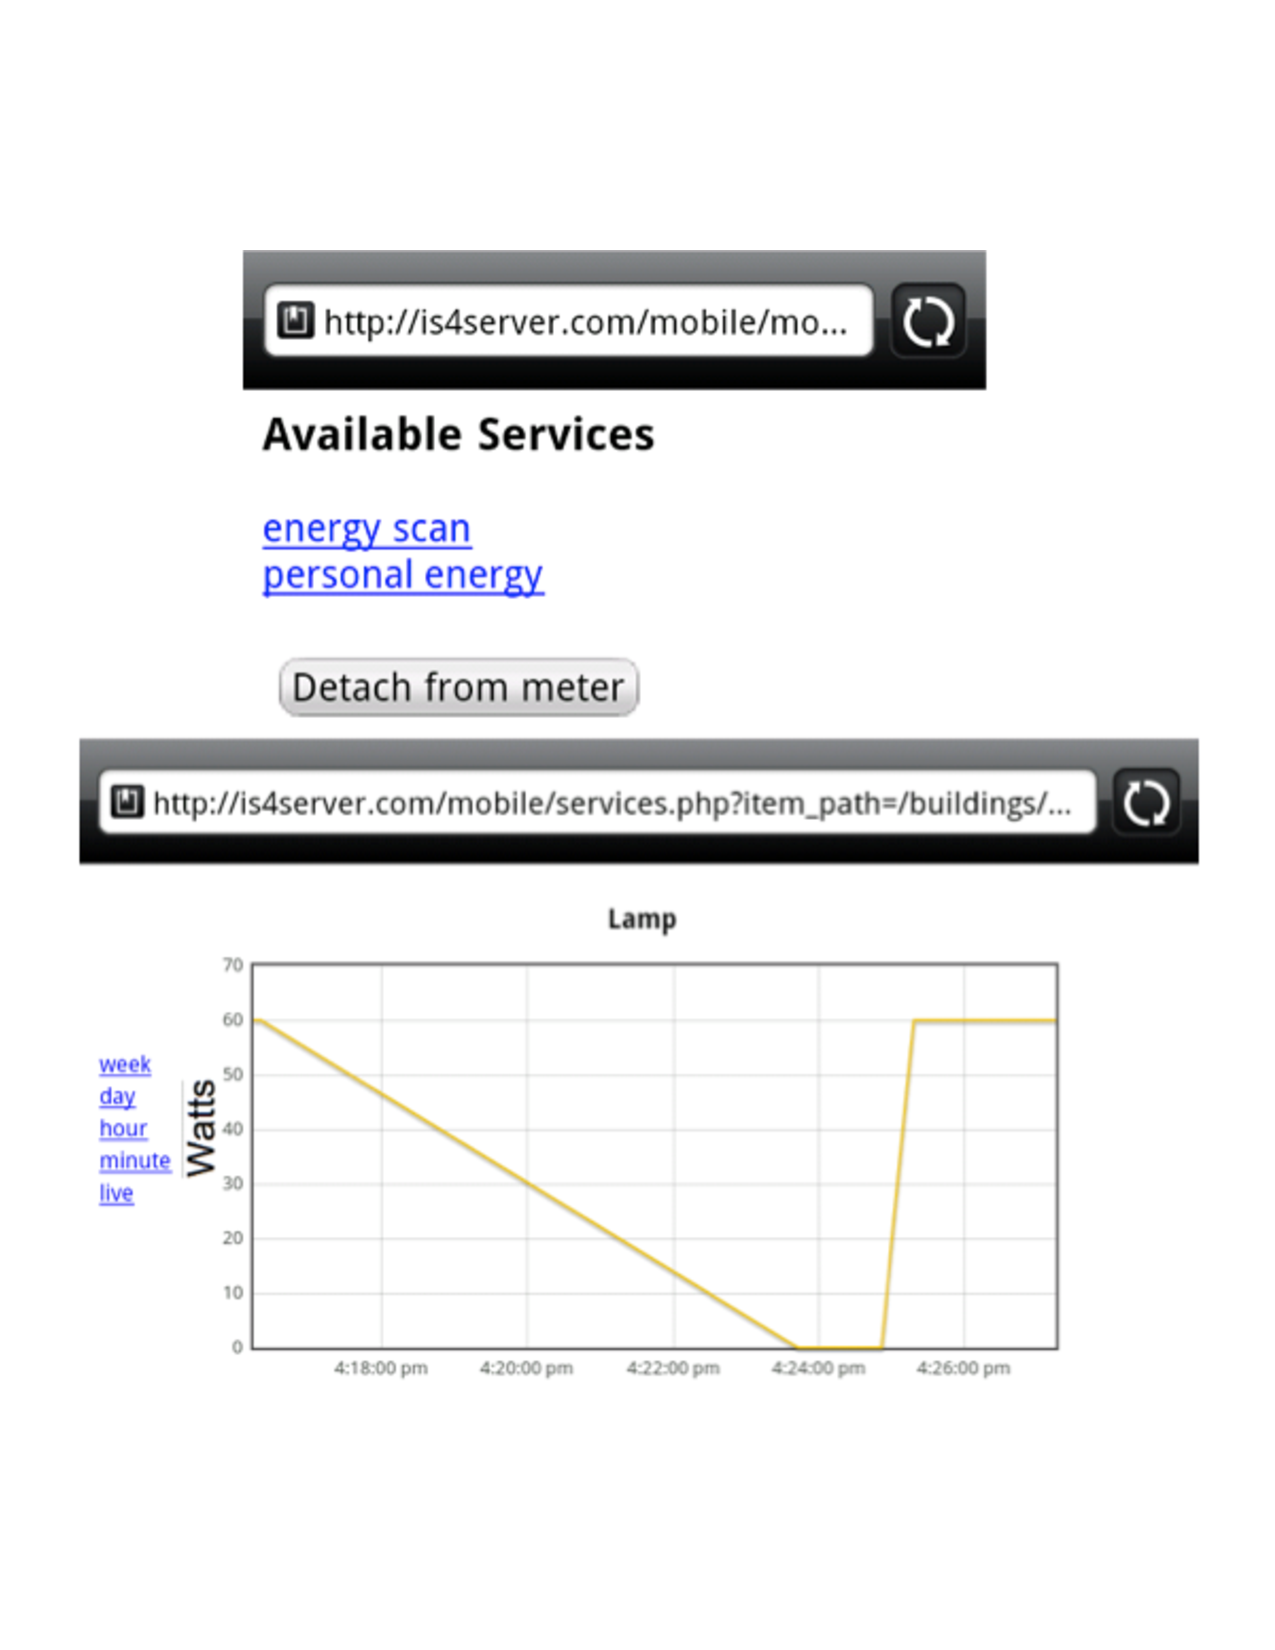
\includegraphics[scale=0.39]{figs/menuenergyscan}
\caption{Item scanner screenshot. Lorem Ipsum is simply dummy text of the printing and typesetting industry. Lorem Ipsum has 
been the industry's standard dummy text ever since the 1500s, when an unknown printer took a galley of 
type and scrambled it to make a type specimen book.  }
\label{fig:itemscanscreen}
\end{center}
\end{figure}

The main thrust of this application revolves around aggregating feeds with respect to the spatial hierarchy that was
constructed for the energy audit.  A person can scan any item from the building and floor down to the room
and individual device.

\subsubsection{Issues}
In addition to the consistency challenges from the energy audit, apportionment is non-trivial.  Even with an accurate
view of where items have been moved, tracking the consituents and calculating aggregate is challenging in real-time.
Since meter clocks are not syncrhonized, the data must be cleaned before an aggregate can even be computed.
We address this problem with dynamic aggregation and discuss the details in section~\ref{sec:dynagg}.

\subsection{Personalized Energy Tracking}
A user identifies themselves with a username and password.  This create a folder in StreamFS with their username.  As they
walk around the building, they can tag items that belong to them by swipe them and clicking `my item' in the mobile
application.  The application records the item and its location when this is done.  A location folder is created
in the user's directory along with a symbolic link to the item that they tagged.  This allows us to aggregate both the totals
by location and totals by user.  Figure~\ref{fig:personalscanscreen} shows the interface for tagging a device 
and the aggregate for the owner of the items.

%FILL IN WITH REAL GRAPH
% \begin{figure}[htb!]
% \begin{center}
% 
\includegraphics[scale=0.39]{figs/blankbox}
% \caption{Personal energy screenshot. Lorem Ipsum is simply dummy text of the printing and typesetting industry. Lorem Ipsum has 
% been the industry's standard dummy text ever since the 1500s, when an unknown printer took a galley of 
% type and scrambled it to make a type specimen book.  }
% \label{fig:personalscanscreen}
% \end{center}
% \end{figure}

\subsection{Issues}
In this application, the main challenge was in localization of a particular user.  In order to form aggregates for the total c
onsumed by the user in a particular sapce, we want to present the user with an aggregate of the items they know in that space.  
To do this automatically one might require indoor localization using the WiFi infrastructure.  However, we leverage the tags infrastructure
and user input to identify who they are and where they are.  With a simple `login' and swipe, they get personlized,
location-specific, aggregate energy consumption data.

\begin{itemize}
\item Mobile objects: objects move and are placed in different locations
\item Changing meters: meters are moved or items are disconnected and re-connected to other meters
\item Aggregation that track constituents over time:  just a description, talk more about it in next section
\end{itemize}